\chapter{Fundamentação Teórica}
\label{cap:fundamentacao}

O objetivo deste capítulo é abordar as bases conceituais e técnicas que precedem e apoiam este trabalho. Inicialmente, caracteriza-se o fenômeno da evolução semântica dos dados, comparando-o com a evolução de esquema. Em seguida, descreve-se o sistema que serve de base que este estudo busca estender, o MellowDB. Por fim, apresentam-se os fundamentos de bancos de dados distribuídos e suas definições, mostrando como o MongoDB lida com múltiplas máquinas.

\section{Evolução de dados: esquema e semântica}
\label{sec:evolucao}
Coleções de dados que perduram por longos períodos podem não manter um mesmo significado, isto é, não há uma garantia de estabilidade. Um mesmo valor pode representar entidades distintas em épocas diferentes, ou uma mesma entidade pode ser representada de várias formas ao longo do tempo. Por exemplo, no caso do Brasil, o município de \textit{Moji Mirim} passou a ter a grafia de \textit{Mogi Mirim} em 2016, assim como o padrão de classificação de causas de óbito migrou da CID-9 para a CID-10 em 1996, alterando tanto os códigos quanto o agrupamento das doenças. Nesse cenário, uma consulta ingênua que filtre por um único nome ou código pode, por consequência, retornar apenas parte dos dados históricos. A Figura~\ref{fig:evolucao-semantica} ilustra esse tipo de mudança semântica.

\begin{figure}[htb]
  \centering
  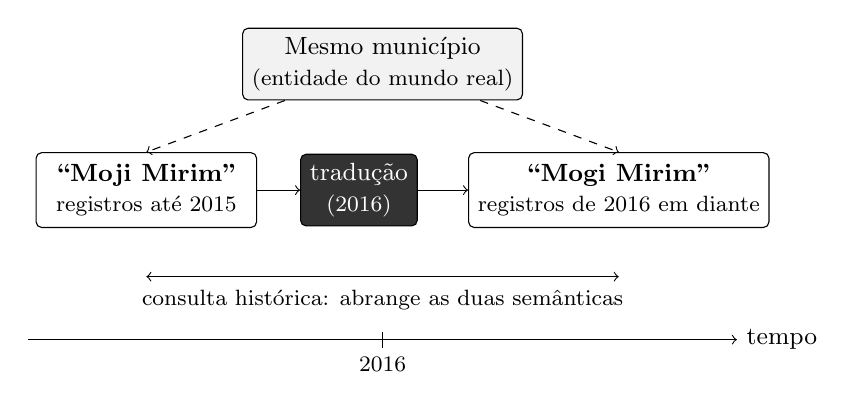
\begin{tikzpicture}[font=\small]
    % entidade do mundo real (referente comum)
    \node[draw, rounded corners=2pt, fill=black!5, align=center, minimum height=0.8cm]
      (ent) at (0,2) {Mesmo município\\\footnotesize (entidade do mundo real)};
    % rótulos antes e depois da evolução
    \node[draw, rounded corners=2pt, align=center, minimum width=2.8cm, minimum height=0.95cm]
      (old) at (-3,0.4) {\textbf{``Moji Mirim''}\\\footnotesize registros até 2015};
    \node[draw, rounded corners=2pt, align=center, minimum width=2.8cm, minimum height=0.95cm]
      (new) at (3,0.4) {\textbf{``Mogi Mirim''}\\\footnotesize registros de 2016 em diante};
    % operação de evolução que marca a mudança de significado
    \node[draw, rounded corners=2pt, fill=black!80, text=white, align=center]
      (op) at (-0.3,0.4) {tradução\\\footnotesize (2016)};
    % ambos os rótulos designam a mesma entidade
    \draw[dashed,->] (ent) -- (old.north);
    \draw[dashed,->] (ent) -- (new.north);
    % o rótulo antigo é transformado no novo pela operação
    \draw[->] (old) -- (op);
    \draw[->] (op) -- (new);
    % eixo do tempo
    \draw[->] (-4.5,-1.5) -- (4.5,-1.5) node[right] {tempo};
    \draw (0,-1.4) -- (0,-1.6) node[below] {\footnotesize 2016};
    % uma consulta histórica abrange as duas semânticas
    \draw[<->] (-3,-0.7) -- (3,-0.7);
    \node at (0,-1.0) {\footnotesize consulta histórica: abrange as duas semânticas};
  \end{tikzpicture}
  \caption[Evolução semântica: a tradução ``Moji Mirim'' para ``Mogi Mirim''.]{%
    Evolução semântica ilustrada pela tradução ``Moji Mirim'' $\rightarrow$
    ``Mogi Mirim'' (2016).}
  \label{fig:evolucao-semantica}
\end{figure}


Sob o termo de \textit{evolução de domínio}, \citet{ventrone1991} apresenta esse fenômeno onde o signicado dos correspondentes, externos ao sistema, dos valores de um domínio mudam ao longo do tempo, fazendo o domínio se tornar um agregado de subdomínios semanticamente incompatíveis, dos quais um simples mapeamento entre valores ``antigos'' e ``novos'' pode não ser suficiente. Dentre as diferentes formas de evolução que ele expõe, há a distinção entre a \textit{heterogeneidade semântica}, onde a semântica dos dados está implícita no código das aplicações, e a heterogeneidade sintática, pois ele argumenta que tornar a informação explícita nos próprios dados faz do problema não mais semântico, mas sim sintático e de fácil solução. Nesse contexto, observa-se que cada mudança de significado produz uma versão distinta dos dados, isto é, um sistema pode adotar o uso de versionamento sobre o domínio, ideia que é trabalhada no sistema base deste trabalho.

Por outro lado, vale destacar a outra parte do desenvolvimento contínuo de um banco de dados, a \textit{evolução de esquema}, na qual a estrutura muda com a adição ou a remoção de atributos e relações. Esse é um campo maduro na literatura e com diversas soluções e maneiras de lidar com o problema em sistemas comerciais. A revisão de \citet{brahmia2024} a definem como a modalidade que adapta os dados existentes a um novo esquema, poupando administradores e programadores desse compromisso, e registra que os SGBDs oferecem suporte apenas limitado e pontual a ela. Embora não faça parte do escopo desta pesquisa, a evolução de esquema é um problema relacionado, cujo campo apresenta fundamentos e soluções incorporados no sistema base do trabalho. 

Há duas estratégias gerais para lidar com dados sob evolução que aparecem recorrentemente na literatura. A primeira, \textbf{ansiosa} (\textit{eager}), converte ou migra os dados no momento em que a mudança ocorre, enquanto a segunda, \textbf{preguiçosa} (\textit{lazy}), mantém os dados em suas versões originais e adia o tratamento para o momento da consulta. \citet{devries2004} enquadram essa escolha como conversão \textit{strict} (ansiosa), \textit{lazy} ou inexistente, quando nenhum alteração é feita. \citet{moon2008}, por exemplo, usa da abordagem preguiçosa para bancos de dados de tempo de transação sob evolução de esquema, criando uma camada que lê a consulta do usuário e a reescreve para comtemplar as equivalências de diferentes versões dos dados. Para representar as mudanças, os autores introduziram operadores de modificação de esquema (\textit{Schema Modification Operators}) que mapeiam versões sucessivas, incluindo a fusão e a divisão de tabelas. Essas são soluções consolidadas no contexto de esquema que serão retomados nessa pesquisa de semântica.

O MellowDB \citep{nepomuceno2026}, sistema base que esta monografia estende, aparece nesse contexto, porém dedicado especificamente à evolução semântica. Ele registra as operações de evolução (tradução, fusão e divisão) na forma de metadados, e oferece as mesmas duas estratégias: a reescrita de consultas (\textit{rewrite}), preguiçosa, e o pré-processamento com versionamento na inserção (\textit{preprocess}), ansioso. Esse sistema será mais detalhado na seção seguinte. 

\section{O sistema base: MellowDB}
\label{sec:mellowdb}

O MellowDB \citep{nepomuceno2026} é uma biblioteca de \textit{middleware}, escrita em Python e distribuída sob a licença MIT, que gerencia a evolução semântica sobre um banco de dados NoSQL orientado a documentos. Ele permite que o usuário consulte uma coleção semanticamente heterogênea como se fosse homogênea, isto é, o sistema o isenta de conhecer as mudanças de significado ocorridas ao longo do tempo e, concomitantemente, preserva a fidelidade das semânticas passadas. A princípio, ele foi concebido para ser executado em um banco de dados de \textit{nó único}, mas suficientemente aberto para desenvolvimento em um sistema distribuído.

O arcabouço permite inserir e processar registro formados por um par de instante de tempo de validade e um conjunto de pares atributo-valor. Uma \textbf{operação de evolução semântica} é um evento discreto e datado que contém uma ocorrência de heterogeneidade semântica, sendo responsável por transformar os valores afetados de um atributo a partir de um dado momento. Aqui, ela se divide em três operações:

\begin{itemize}
  \item \textbf{Tradução:} substitui um valor por outro e é reversível (Figura~\ref{fig:evolucao-semantica});
  \item \textbf{Fusão:} reúne vários valores em um só e só pode ser aplicada no sentido direto do tempo;
  \item \textbf{Divisão:} separa um valor em vários e, de modo simétrico, só pode ser aplicada no sentido reverso.
\end{itemize}

Esses três casos correspondem a transformações reais: a mudança do nome da cidade, a fusão da Guanabara com o Rio de Janeiro (1975) e a cisão de Laguna em Laguna e Pescaria Brava (2013); a Figura~\ref{fig:fusao-divisao} ilustra as duas últimas.

\begin{figure}[H]
  \centering
  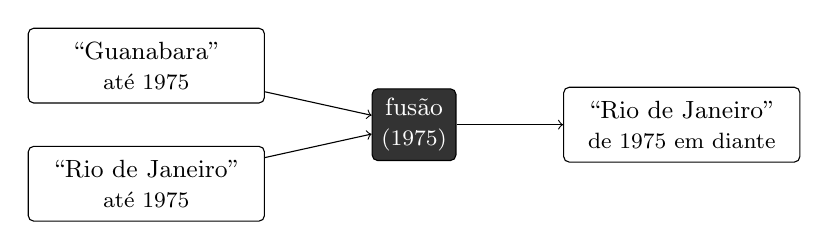
\begin{tikzpicture}[font=\small,
      rec/.style={draw, rounded corners=2pt, align=center, minimum width=3cm, minimum height=0.95cm},
      op/.style={draw, rounded corners=2pt, fill=black!80, text=white, align=center}]
    \node[rec] (a)  at (-3.4, 0.75) {``Guanabara''\\\footnotesize até 1975};
    \node[rec] (b)  at (-3.4,-0.75) {``Rio de Janeiro''\\\footnotesize até 1975};
    \node[op]  (op) at (0,0) {fusão\\\footnotesize (1975)};
    \node[rec] (c)  at (3.4,0) {``Rio de Janeiro''\\\footnotesize de 1975 em diante};
    \draw[->] (a) -- (op);
    \draw[->] (b) -- (op);
    \draw[->] (op) -- (c);
  \end{tikzpicture}

  {\footnotesize (a) \textbf{Fusão}: vários valores passam a um só; operação de sentido único.}

  \vspace{3ex}

  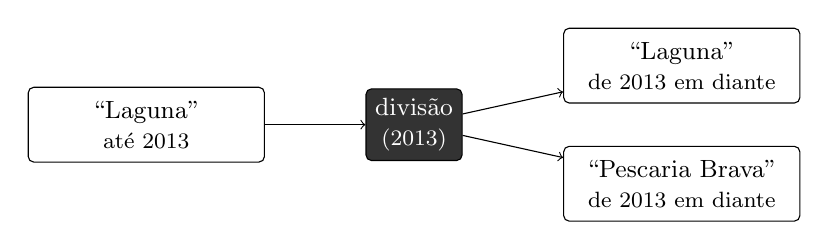
\begin{tikzpicture}[font=\small,
      rec/.style={draw, rounded corners=2pt, align=center, minimum width=3cm, minimum height=0.95cm},
      op/.style={draw, rounded corners=2pt, fill=black!80, text=white, align=center}]
    \node[rec] (a)  at (-3.4,0) {``Laguna''\\\footnotesize até 2013};
    \node[op]  (op) at (0,0) {divisão\\\footnotesize (2013)};
    \node[rec] (c1) at (3.4, 0.75) {``Laguna''\\\footnotesize de 2013 em diante};
    \node[rec] (c2) at (3.4,-0.75) {``Pescaria Brava''\\\footnotesize de 2013 em diante};
    \draw[->] (a) -- (op);
    \draw[->] (op) -- (c1);
    \draw[->] (op) -- (c2);
  \end{tikzpicture}

  {\footnotesize (b) \textbf{Divisão}: um valor passa a vários; operação de sentido único.}
  \caption[Fusão e divisão como operações de evolução semântica.]{%
    Na fusão (a), uma consulta pelo nome novo deve alcançar também os registros das origens. Na divisão (b), uma consulta pelo nome antigo deve alcançar os fragmentos.}
  \label{fig:fusao-divisao}
\end{figure}

Como visto anteriormente, o MellowDB oferece duas estratégias para lidar com essas operações. A primeira, reescrita de consultas (\textit{rewrite}), lê os metadados das operações para reescrever a consulta formulada pelo usuário delimitando cláusulas por tempo e combinando-as por disjunção, isto é, uma parte da consulta para cada versão afetada. Ao final, os campos afetados pelas operações, dos registros recuperados, são projetados para a semântica mais recente, porém sem alterar os dados armazenados. Entretanto, na segunda estratégia, pré-processamento (\textit{preprocess}), o tratamento dos dados ocorre na inserção, seja de um registro ou da própria operação nova. Nessa abordagem, a informação adicionada é materializada em todas as versões semânticas e armazenada já reconciliada. Ao inserir uma nova operação, todos os registros existentes são reprocessados.

Nos exemplos das Figuras ~\ref{fig:evolucao-semantica} e ~\ref{fig:fusao-divisao} (a), a reescrita tem os seguintes resultados:
\begin{flalign}
  & \phantom{\rightarrow\;} \text{municipio} = \text{``Mogi Mirim''} \nonumber & \\
  & \rightarrow\; (\text{municipio} = \text{``Mogi Mirim''} \land \text{ano} \ge 2016) \lor \nonumber & \\
  & \phantom{\rightarrow\;} (\text{municipio} = \text{``Moji Mirim''} \land \text{ano} < 2016) &
\end{flalign}
\begin{flalign}
  & \phantom{\rightarrow\;} \text{estado} = \text{``Rio de Janeiro''} \nonumber & \\
  & \rightarrow\; (\text{estado} \in \text{\{``Rio de Janeiro'', ``Guanabara''\}} \land \text{ano} < 1975) \lor \nonumber & \\
  & \phantom{\rightarrow\;} (\text{estado} = \text{``Rio de Janeiro''} \land \text{ano} \ge 1975) &
\end{flalign}

A eficiência dessas soluções é regida pelo armazenamento de três coleções:
\begin{itemize}
  \item A \textbf{coleção bruta} guarda os registros originais sem alteração, preservando o histórico e a versão original de cada dado;
  \item A \textbf{coleção de versões semânticas} contém apenas os metadados das operações, organizados como uma lista duplamente ligada de versões, assim cada versão conhece a operação que a leva à próxima e à anterior;
  \item A \textbf{coleção processada}, usada somente pela estratégia ansiosa, guarda as versões materializadas, mas associa a cada registro um intervalo de versões em que ele é válido, de modo que registros não afetados por uma operação não precisem ser duplicados.
\end{itemize}


\begin{figure}[H]
  \centering
  \begin{minipage}[t]{0.47\textwidth}
\begin{lstlisting}[language=,basicstyle=\ttfamily\scriptsize,frame=single,numbers=none,columns=fullflexible,keepspaces=true,showstringspaces=false]
{
  "estado": "Guanabara",
  "ano": 1975,
  "populacao": 4857700,
  "_original_id": "a4d8",
  "_min_version_number": "-inf",
  "_max_version_number": 2,
  "_evoluted": false
}
\end{lstlisting}
    \centerline{\footnotesize (a) cópia anterior à fusão}
  \end{minipage}\hfill
  \begin{minipage}[t]{0.47\textwidth}
\begin{lstlisting}[language=,basicstyle=\ttfamily\scriptsize,frame=single,numbers=none,columns=fullflexible,keepspaces=true,showstringspaces=false]
{
  "estado": "Rio de Janeiro",
  "ano": 1975,
  "populacao": 4857700,
  "_original_id": "a4d8",
  "_min_version_number": 2,
  "_max_version_number": "+inf",
  "_evoluted": true
}
\end{lstlisting}
    \centerline{\footnotesize (b) cópia posterior à fusão}
  \end{minipage}
  \caption[Documentos da coleção processada.]{%
    Dois documentos da coleção processada para um registro inserido como ``Guanabara'' (1975), sob a fusão da Guanabara com o Rio de Janeiro. A estratégia ansiosa materializa o registro em uma cópia por intervalo de versões \texttt{[\_min\_version\_number, \_max\_version\_number)}. A cópia anterior mantém ``Guanabara'' e a posterior já carrega ``Rio de Janeiro'', ambas apontando para o mesmo registro bruto (\texttt{\_original\_id}). Um registro não afetado por nenhuma operação ocuparia um único intervalo, de \texttt{-inf} a \texttt{+inf}, sem duplicação. Valores meramente ilustrativos.}
  \label{fig:colecao-processada}
\end{figure}

Cada operação registrada acrescenta um nó à cadeia de versões, que guarda o tipo da operação, o campo afetado e os valores de origem e destino, ligando a nova versão à anterior e à seguinte (Figura~\ref{fig:cadeia-versoes}). Os números de versão são apenas ordenáveis, de modo que uma operação possa ser inserida entre duas já existentes. No pré-processamento, inserir um registro já o decompõe nas cópias de que ele precisa (Figura~\ref{fig:colecao-processada}), obtidas pela aplicação sucessiva das operações referentes (modo \textit{operations-first}) a ele e verificadas em cascata. Definir uma operação quando os dados já existem (modo \emph{insertion-first}) leva ao reprocessamento das cópias afetadas.

\begin{figure}[H]
  \centering
  \begin{minipage}[t]{0.47\textwidth}
\begin{lstlisting}[language=,basicstyle=\ttfamily\scriptsize,frame=single,numbers=none,columns=fullflexible,keepspaces=true,showstringspaces=false]
{
  "version_number": 1,
  "version_valid_from": "0001-01-01",
  "previous_version": null,
  "previous_operation": null,
  "next_version": 2,
  "next_operation": {
    "type":  "translation",
    "field": "municipio",
    "from":  "Moji Mirim",
    "to":    "Mogi Mirim"
  }
}
\end{lstlisting}
    \centerline{\footnotesize (a) versão inicial}
  \end{minipage}\hfill
  \begin{minipage}[t]{0.47\textwidth}
\begin{lstlisting}[language=,basicstyle=\ttfamily\scriptsize,frame=single,numbers=none,columns=fullflexible,keepspaces=true,showstringspaces=false]
{
  "version_number": 2,
  "version_valid_from": "2016-01-01",
  "previous_version": 1,
  "previous_operation": {
    "type":  "translation",
    "field": "municipio",
    "from":  "Mogi Mirim",
    "to":    "Moji Mirim"
  },
  "next_version": null,
  "next_operation": null
}
\end{lstlisting}
    \centerline{\footnotesize (b) após a tradução (2016)}
  \end{minipage}
  \caption[Documentos da cadeia de versões semânticas.]{%
    Dois documentos da coleção de versões semânticas para a tradução ``Moji Mirim'' $\rightarrow$ ``Mogi Mirim'' (2016). Cada documento guarda a operação que o liga à versão anterior e à seguinte, ou seja, o tipo, campo afetado e valores de origem e destino, formando uma lista duplamente ligada. Campos auxiliares no sistema foram omitidos.}
  \label{fig:cadeia-versoes}
\end{figure}


Na implementação, o MellowDB é escrito em Python com uma interface que espelha a do PyMongo, o \textit{driver} oficial do MongoDB. O processamento semântico é executado dentro do próprio SGBD, por meio de \textit{pipelines} de agregação do MongoDB, e não no cliente, para controlar o uso de memória em coleções grandes. O MongoDB foi escolhido, entre os bancos orientados a documentos, por armazenar metadados junto aos dados, pela licença aberta, pela atividade da comunidade e pelo suporte a agregação. O protótipo do sistema prioriza as operações dominantes em coleções históricas de longa duração, inserções e consultas, deixando atualizações e remoções como trabalho futuro e que fogem do escopo da extensão dessa monografia.

A avaliação do sistema, conduzida sobre dados reais de mortalidade do DATASUS (a transição da CID-9 para a CID-10)\footnote{O conjunto de dados, configurado para essa análise do MellowDB, está disponível em: NEPOMUCENO, P. I. S.; BRAGHETTO, K. \textit{Dataset for Evaluating Semantic Evolution Handling in MellowDB: Query Rewriting vs. Data Preprocessing}. Mendeley Data, V1, 2025. DOI: \url{10.17632/ytfdw568kk.1}.}, mostra que as duas estratégias são viáveis em produção, onde cada uma superior em casos diferentes. A reescrita vence em cargas dominadas por escrita, enquanto o pré-processamento vence nos demais cenários, com a indexação estreitando a diferença entre elas \citep{nepomuceno2026}. Entretanto, esse projeto e análise foram feitos em um único nó, algo que os autores apontaram como trabalho futuro em direcionar ao ambiente distribuído com coleções eventualmente replicadas e particionadas.

% \section{Bancos de dados distribuídos}
% \label{sec:distribuidos}
%
% \section{MongoDB distribuído}
% \label{sec:mongodb}